\chapter{Autoregulon Networks: COMING SOON}
\label{ch-autoregulons}

Appendix \ref{ch-genomics-vocab}

\section{Autoregulon net motif}

\begin{figure}[h!]
$$
\xymatrix{
&\rvx\ar[dd]|{-\alp}\ar[dl]
\\
f(\rvx)\ar[dr]|{1}
\\
&\Circle{\frac{d\rvx}{dt}}
}\quad
\xymatrix{\\=}
\quad
\xymatrix{
\\
\rvx\ar@{=>}[d]
\\
\dot{\rvx}
}
$$
\caption{Autoregulon net motif and the symbol we will
use to denote it when we consider
networks of connected autoregulons. Assume $\alp >0$.}
\label{fig-net-motif}
\end{figure}

\beq
\frac{dx}{dt}=f(x)-\alp x
\eeq

\beq
f(x)=\left\{
\begin{array}{ll}
\beta\indi(x<K)
&(f \text{ is lowpass})
\\
\beta\indi(x>K)
&(f \text{ is highpass})
\end{array}
\right.
\eeq
where $\alp, \beta > 0$

\beq
x= \underbrace{x_0 e^{-\alp t}}_{x_h} +
\underbrace{f(x)
\left[ \frac{1-e^{-\alp t}}{\alp}\right]}_{x_p}
\eeq

Hmomogeneous ($x_h$) and particular ($x_p$)
solution for the autoregulon
first order  differential equation.
The homogenoeus solution depends on the initial conditions $x_0$. The geneneral solution
is a sum of $x_h$ and $x_p$.

Three $x$ values $\{x_0, K, \frac{\beta}{\alp}\}$, and
two $f$ values $\{ \text{lowpass, highpass}\}$

\begin{figure}[h!]
\centering
\includegraphics[width=3in]
{gene_reg_net/autoreg-approxs.png}
\caption{Approximations that we use to understand the
gross behavior of the autoregulon.
 }
\label{fig-autoreg-lowpass}
\end{figure}

\begin{figure}[h!]
\centering
\includegraphics[width=4in]
{gene_reg_net/autoreg-lowpass.png}
\caption{$x_h$ and $x_p$ of autoregulon for lowpass $f$}
\label{fig-autoreg-lowpass}
\end{figure}

\begin{figure}[h!]
\centering
\includegraphics[width=4in]
{gene_reg_net/autoreg-highpass.png}
\caption{$x_h$ and $x_p$ of autoregulon  for highpass $f$}
\label{fig-autoreg-lowpass}
\label{fig-autoreg-highpass}
\end{figure}


\section{Multiple autoregulons}

\beq
\cala x = 0\;,\;\; \text{ where } \cala=
\frac{d}{dt} + \alp - \frac{f(x)}{x}
\eeq





\begin{figure}[h!]
$$
\xymatrix@C=6pc{
\rvx \ar@{=>}[dd]\ar[ddr]^<<<<{\gamma_{\rvy|\rvx}}
& \rvy \ar@{=>}[dd]\ar[ddl]_<<<<{\gamma_{\rvx|\rvy}}
\\
&
\\
\dot{\rvx}
&\dot{\rvy}
}
\xymatrix{\\
\quad=\quad}
\xymatrix@C=5pc{
\\
\Rect{\rvx}
\autoar{r}
{\gamma_{\rvy|\rvx}}
{\gamma_{\rvx|\rvy}}
&
\Rect{\rvy}}
$$
\caption{Two autoregulons connected to each other.}
\label{fig-2-autoregulons}
\end{figure}

\beq
\left\{
\begin{array}{l}
\cala\rvx = \gamma_{\rvx|\rvy}\;\rvy
\\
\cala\rvy = \gamma_{\rvy|\rvx}\;\rvx
\end{array}
\right.
\eeq


\begin{figure}[h!]
$$
\xymatrix@C=4pc@R=5pc{
&\Rect{\rvx}
\autoar{ld}{}{}
\autoar{rd}{}{}
\\
\Rect{\rvy}\autoar{rr}{}{}
&&
\Rect{\rvz}
}
$$
\caption{Three autoregulons connected to each other.
$\gamma_{\rvx|\rvy}$ coefficients are left implicit.}
\label{fig-3-autoregulons}
\end{figure}


\beq
\left\{
\begin{array}{l}
\cala\rvx =
\gamma_{\rvx|\rvy}\;\rvy
+
\gamma_{\rvx|\rvz}\;\rvz
\\
\cala\rvy =
\gamma_{\rvy|\rvx}\;\rvx
+
\gamma_{\rvy|\rvz}\;\rvz
\\
\cala\rvz =
\gamma_{\rvz|\rvx}\;\rvx
+
\gamma_{\rvz|\rvy}\;\rvy
\end{array}
\right.
\eeq

Use $\xymatrix{\rvx\ar[r]^{+}&\rvy}$
to denote
$\xymatrix{\rvx\ar[r]^\alp&\rvy}$
with $\alp>0$.

Use $\xymatrix{\rvx\ar[r]^{-}&\rvy}$
to denote
$\xymatrix{\rvx\ar[r]^\alp&\rvy}$
with $\alp<0$

Use $\xymatrix{\rvx\ar[r]^{0}&\rvy}$
to denote
$\xymatrix{\rvx\ar[r]^\alp&\rvy}$
with $\alp=0$.

\begin{figure}[h!]
$$
\begin{array}{ccc}
\xymatrix@C=4pc@R=5pc{
&\Rect{\rvx}
\autoar{ld}{-}{0}
\autoar{rd}{+}{0}
\\
\Rect{\rvy}\autoar{rr}{-}{0}
&&
\Rect{\rvz}
}
&&
\xymatrix@C=4pc@R=5pc{
&\Rect{\rvx}
\autoar{ld}{-}{0}
\autoar{rd}{+}{0}
\\
\Rect{\rvy}\autoar{rr}{+}{0}
&&
\Rect{\rvz}
}
\\
\\
(a)&&(b)
\end{array}
$$
\caption{$(a)$ shows a coherent net of 3 autoregulons because $\sign(\gamma_{\rvz|\rvy}\gamma_{\rvy|\rvx})=\sign(\gamma_{\rvz|\rvx})$.
$(b)$ shows a incoherent net of 3 autoregulons because $\sign(\gamma_{\rvz|\rvy}\gamma_{\rvy|\rvx})\neq \sign(\gamma_{\rvz|\rvx})$.
}
\label{fig-3-coherent-autoregulons}
\end{figure}



\section{Single Input Module (SIM) net}

\section{Feedforward Loop (FFL) net}

\section{Bistable net}

\section{Biological clock net}